\chapter{Result and Discussion}

\begin{figure}
	\begin{subfigure}{8cm}
		\centering    
    	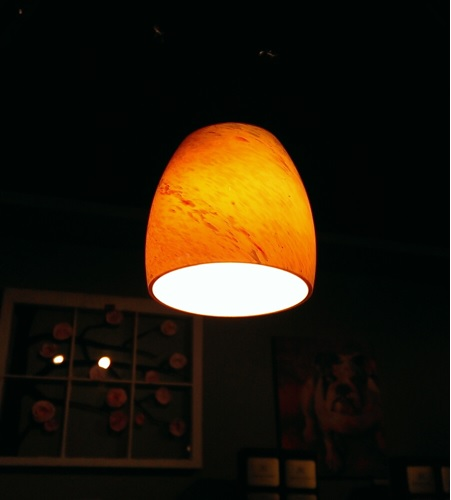
\includegraphics[width=7cm,height=9cm,keepaspectratio]{images/ch5/bulb_input.jpg}
    	\caption{} 
    \end{subfigure}
  	\begin{subfigure}{6cm}
  		\centering
  		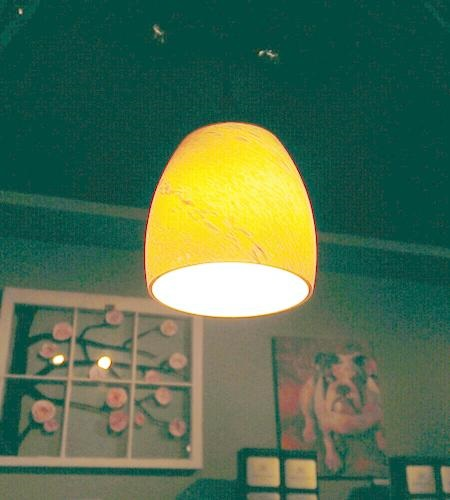
\includegraphics[width=7cm,height=9cm,keepaspectratio]{images/ch5/bulb_ssr.jpg}
   		\caption{}
  	\end{subfigure}
  	\caption{a) Input Image b)Enhanced Image using SSR}
  	\label{fig:ssr}
\end{figure}

\begin{figure}
	\begin{subfigure}{8cm}
		\centering    
    	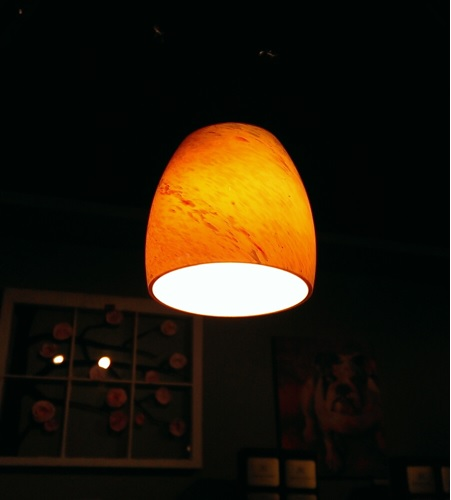
\includegraphics[width=7cm,height=9cm,keepaspectratio]{images/ch5/bulb_input.jpg}
    	\caption{} 
    \end{subfigure}
  	\begin{subfigure}{6cm}
  		\centering
  		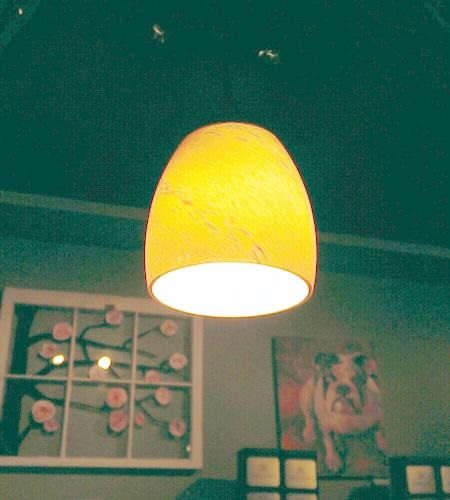
\includegraphics[width=7cm,height=9cm,keepaspectratio]{images/ch5/bulb_msr.jpg}
   		\caption{}
  	\end{subfigure}
  	\caption{a) Input Image b)Enhanced Image using SSR}
  	\label{fig:msr}
\end{figure}
